\documentclass[10pt,twocolumn,letterpaper]{article}

\usepackage[pagenumbers]{cvpr}
\usepackage{booktabs}
\usepackage{graphicx}
\usepackage{amsmath}
\usepackage{multirow}

\definecolor{cvprblue}{rgb}{0.21,0.49,0.74}
\usepackage[pagebackref,breaklinks,colorlinks,allcolors=cvprblue]{hyperref}

\def\paperID{3201}
\def\confName{CVPR}
\def\confYear{2026}

\title{Generative Sparse-View 3D Reconstruction\\
with Frozen-Pose Gaussian Splatting}

\author{Yuming Zhang\\
The Hong Kong University of Science and Technology (Guangzhou)\\
{\tt\small yzhang395@connect.hkust-gz.edu.cn}
}

\begin{document}
\maketitle

\begin{abstract}
We study sparse-view 3D reconstruction on three course scenes: Waymo-405841, DL3DV-2, and Re10k-1.
Part~1 freezes the poses of COLMAP and VGGT and trains standard 3D Gaussian Splatting for 30{,}000 iterations.
VGGT-$\Omega$ weights are gated, so that initializer is recorded as a failure and is not silently skipped.
Part~2 runs i3dgs on dense and sparse views with dataset intrinsics and no ground-truth extrinsics.
Part~3 exports the sparse i3dgs Gaussians, inserts two GeoQuery rounds at iterations 1500 and 3000, and compares them with a sparse-only control.
Test views never enter training.
Rendering scores use a 500-step evaluation pose.
On Waymo, VGGT at 30k reaches 22.25\,dB PSNR against 11.99\,dB for COLMAP, while COLMAP remains stronger on DL3DV (28.16 vs.\ 25.03\,dB).
Dense i3dgs drops most views on DL3DV and Re10k.
On all three scenes, the closed loop does not beat its sparse-only control after the 3000-iteration opacity reset.
Code and run instructions: \url{https://github.com/Oliver-ming/Intro_to_CV_project_4}.
\end{abstract}

\section{Introduction}
Sparse-view reconstruction has to answer two questions that a dense video hides.
The first is where the cameras are.
The second is what the scene looks like between the cameras that were actually captured.
Classical structure from motion answers the first question by matching and bundle adjustment~\cite{agarwal2011rome}.
Feed-forward geometry models answer it with one network pass~\cite{wang2025vggt,wang2026omega,lin2025da3}.
Radiance-field training then turns those cameras and points into a renderable scene~\cite{kerbl20233dgs}.
When the captured views are far apart, the optimized field still leaves holes, and image diffusion has been used to invent the missing observations~\cite{cao2026geoquery,wu2025difix,wu2025genfusion,yin2025gsfixer,zhao2026brpo}.

This report follows that split on the three mandatory scenes.
Part~1 asks whether a foundation model is a better initializer than COLMAP when both are followed by the same 3D Gaussian Splatting (3DGS) budget.
Part~2 removes ground-truth extrinsics and compares dense and sparse i3dgs runs~\cite{meuleman2026i3dgs}.
Part~3 asks whether two rounds of geometry-conditioned diffusion, written back as extra training views, improve the sparse reconstruction.
Generated views are not fed back into i3dgs.
Poses stay frozen after initialization.

The implementation choices that affect the numbers are stated with the method.
The most important ones are the evaluation pose, the treatment of views i3dgs never registers, and the fact that VGGT-$\Omega$ could not be run.

\section{Related Work}
Kerbl~\etal~\cite{kerbl20233dgs} represent a scene as anisotropic 3D Gaussians and rasterize them in real time.
Later variants change the primitive or the frequency content~\cite{lu2024scaffold,zhao2025wavelet}.
Those variants are not the optimizer used here.
Every Part~1 and Part~3 reconstruction uses the official 3DGS training loop, the same iteration budget, and frozen poses.

COLMAP remains the classical initializer~\cite{agarwal2011rome}.
VGGT replaces matching and bundle adjustment with a transformer that predicts cameras and depth from the whole set of frames~\cite{wang2025vggt}.
VGGT-$\Omega$ scales that model~\cite{wang2026omega}.
Depth Anything~3 estimates metric depth and cameras from images~\cite{lin2025da3}.
Streaming variants process long videos without a single joint forward~\cite{chen2026lingbot,cheng2026horizon}.
We use VGGT's joint forward and Depth Anything~3 only as a monocular depth reference inside the closed loop.

Unposed reconstruction is a different problem.
i3dgs registers unordered images and builds Gaussians without a separate SfM stage~\cite{meuleman2026i3dgs}.
Monocular Gaussian SLAM systems such as S3PO-GS and HI-SLAM2 target sequential outdoor or indoor video~\cite{cheng2025s3po,zhang2025hislam}.
We take i3dgs as the Part~2 method and do not run a SLAM baseline.

Generative sparse-view methods invent images at unseen poses and supervise the field with them.
Difix3D+ and GSFixer use single-step or video diffusion as a prior~\cite{wu2025difix,yin2025gsfixer}.
GenFusion closes a loop between reconstruction and generation through video~\cite{wu2025genfusion}.
BRPO studies pseudo-view enhancement for unposed sparse inputs~\cite{zhao2026brpo}.
GeoQuery conditions a diffusion model on a rendered target, a reference image, and a reference depth~\cite{cao2026geoquery}.
We use GeoQuery for the restoration step and keep the 3DGS optimizer, rather than the gsplat trainer shipped with that paper.

\section{Method}
\subsection{Scenes, splits, and resolution}
The mandatory scenes are Waymo-405841~\cite{sun2020waymo}, DL3DV-2~\cite{ling2024dl3dv}, and Re10k-1.
Waymo is an outdoor driving clip.
DL3DV-2 is an outdoor handheld clip, cut to the first 300 frames of the course archive.
Re10k-1 is an indoor clip of 279 frames.
The course video file in the Re10k archive is not a frame and is not imported.

A test view is held out of every initializer, of i3dgs, of GeoQuery, and of the photometric loss.
Waymo test indices satisfy $i \bmod 10 = 5$.
DL3DV and Re10k test indices satisfy $i \bmod 30 = 15$.
Dense views are all remaining captured frames.
Sparse views keep every 10th Waymo frame and every 30th frame of the other two scenes.
If an image is wider than 1600 pixels, the width is rescaled to 1600 and the height follows the aspect ratio.
Otherwise the native resolution is kept.
COLMAP, VGGT, i3dgs, and 3DGS share those pixels.
Waymo therefore trains at $1600\times1067$.
DL3DV and Re10k stay at $256\times256$.
Waymo has 199 frames: 179 dense, 20 sparse, and 20 test.
DL3DV has 300 frames: 290 dense, 10 sparse, and 10 test.
Re10k has 279 frames: 270 dense, 10 sparse, and 9 test.

\subsection{Part 1: frozen-pose initialization}
COLMAP estimates poses and a sparse cloud, then 3DGS trains for 30{,}000 iterations with the viewer disabled and pose optimization off.
Waymo uses the dataset distortion model.
The resulting cameras are undistorted to a pinhole model before 3DGS.
On this COLMAP build the undistorted image is $1599\times1059$, not the prepared $1600\times1067$, and scoring renders at the undistorted size.
DL3DV and Re10k are already pinhole.
Fractional intrinsics in the course camera files are converted to pixels by multiplying by the prepared width.

VGGT runs the public demo without bundle adjustment.
Frame attention does not mix frames, so it is evaluated in chunks of eight frames.
Global attention does mix frames.
On 179 Waymo frames the joint forward fits in one 24\,GB GPU after the image batch is released during attention.
On 270 and 290 frames the full query, key, and MLP activations do not fit.
For those two scenes the weights are stored in bfloat16, global attention is computed in blocks of 2048 tokens with an online softmax, and the MLP is applied in token chunks and written back in place.
A 64-token check against the unblocked attention, with the same weights and rotary embeddings, has a maximum absolute error of $1.8\times10^{-7}$.
Keys and values are still the keys and values of every frame.
The block size changes memory, not the set of frames that interact.
VGGT-$\Omega$ is a gated Hugging Face repository.
This machine is not logged in, and the download returns HTTP 401.
No scene is initialized from it.

Both successful initializers then train the same 3DGS schedule.
Checkpoints and metrics are recorded at 7{,}000 and 30{,}000 iterations.
Initialization time is the wall clock until the COLMAP or VGGT model is written.
Reconstruction time is only the 3DGS loop.
The two clocks are never added together.

\subsection{Part 2: unposed dense and sparse i3dgs}
i3dgs receives images and the dataset focal length.
Ground-truth extrinsics are not passed.
The viewer is disabled.
A view that i3dgs never registers is a dropped view.
Dropped views are excluded from the pose error and are counted.
Pose error is a Sim(3) alignment of camera centers, followed by translation RMSE, on registered training views only.
If fewer than two training views register, Part~3 is a failure.
Every split in this report registered at least five views, so Part~3 is allowed.
The joint reconstruction time is the whole i3dgs process.
i3dgs does not use the 7k/30k 3DGS budget.

Rendering metrics are computed on the exported i3dgs Gaussians, not on a further 30k training run.
Leaves of the hierarchy are kept.
Points that sit far outside the cameras, or that have a huge scale, are removed because they overflow the 3DGS rasterizer.
Cameras and Gaussians are then recentered and scaled into a unit scene.
The export is a standard 3DGS checkpoint at iteration 0.

\subsection{Part 3: two generation rounds and a control}
The sparse export is the start of both the closed loop and the control.
The control trains 30{,}000 iterations on the sparse views only.
The closed loop uses the same Gaussians and the same frozen poses, and it inserts generated views at two fixed iterations.
Because the official trainer reloads cameras from disk, the schedule is three resumed runs: train to 1500 and insert round one, train to 3000 and insert round two, then train through 30{,}000.
Checkpoints are scored at 1500, 3000, 4500, 7000, and 30{,}000.
Generated views are not sent back to i3dgs.

A target pose is the midpoint between two adjacent training poses: translation is interpolated, rotation is slerped.
Round two may pair a real view with a view generated in round one.
GeoQuery restores the image rendered at that pose.
On Waymo the rendered view is 1600 pixels wide.
The SD-Turbo UNet at that size asks for more than the free memory on a 24\,GB GPU, so both the render and the reference are restored with the long side set to 512 and the result is resampled back to the camera size.
Intrinsics are scaled with that resize.
DL3DV and Re10k are already 256 pixels wide, so they are unchanged.
The reference view is the nearest training view by camera center.
Depth Anything~3 runs on that reference image only.
Its depth is resized to the rendered depth and multiplied by the median ratio of the two maps on pixels where both are positive and finite.
Photometric supervision of generated and captured views uses equal weight.
There is no confidence mask.
The public GeoQuery file contains only the \texttt{down\_1} modules and a $3\times3$ position table, so the loader uses neighborhood size 3 and the low-resolution blocks.
Generation time is the wall clock of Depth Anything~3 and GeoQuery.
It is not included in the reconstruction clock.

\subsection{Evaluation pose}
Test images are compared at an evaluation pose, not at the ground-truth test camera.
The reconstruction is frozen.
Each test camera starts at the registered training pose whose frame index is closest.
Only that camera is updated, for 500 Adam steps, by the photometric loss on its own test image.
The official 3DGS rasterizer does not back-propagate into the camera, and the scoring renderer detaches color.
When the loss has no gradient, the six-dimensional pose step is a forward difference with step size $10^{-3}$.
Sim(3) is used only for the training-view pose error.
It is not used to warp ground-truth test cameras.

LPIPS uses a VGG backbone~\cite{zhang2018lpips} and is computed one image at a time.
A batch of Waymo-width images does not fit beside the renderer.

\section{Experiments}
\subsection{Part 1}
Table~\ref{tab:part1} reports 7k and 30k rendering scores, Sim(3) pose error on the training views, and the two clocks.
Figure~\ref{fig:part1} shows the 30k PSNR.
VGGT-$\Omega$ has no row of numbers.
The failure is the same for all three scenes: the checkpoint cannot be downloaded without an approved login.

\begin{table*}[t]
\centering
\small
\setlength{\tabcolsep}{4pt}
\begin{tabular}{llrrrrrr}
\toprule
Scene & Init. & PSNR$\uparrow$ & SSIM$\uparrow$ & LPIPS$\downarrow$ & ATE$\downarrow$ & Init.~s & Recon.~s \\
\midrule
\multirow{2}{*}{Waymo} & COLMAP 7k & 12.28 & 0.434 & 0.590 & 4.020 & 10450 & 1762 \\
 & COLMAP 30k & 11.99 & 0.425 & 0.591 & 4.020 & 10450 & 1762 \\
 & VGGT 7k & 22.81 & 0.775 & 0.470 & 1.115 & 237 & 2030 \\
 & VGGT 30k & 22.25 & 0.753 & 0.434 & 1.115 & 237 & 2030 \\
\midrule
\multirow{2}{*}{DL3DV} & COLMAP 7k & 24.22 & 0.848 & 0.166 & 0.006 & 953 & 770 \\
 & COLMAP 30k & 28.16 & 0.901 & 0.091 & 0.006 & 953 & 770 \\
 & VGGT 7k & 23.86 & 0.802 & 0.209 & 0.035 & 4712 & 413 \\
 & VGGT 30k & 25.03 & 0.824 & 0.167 & 0.035 & 4712 & 413 \\
\midrule
\multirow{2}{*}{Re10k} & COLMAP 7k & 12.68 & 0.397 & 0.414 & 0.011 & 1557 & 452 \\
 & COLMAP 30k & 12.69 & 0.405 & 0.412 & 0.011 & 1557 & 452 \\
 & VGGT 7k & 12.53 & 0.356 & 0.521 & 0.066 & 4733 & 518 \\
 & VGGT 30k & 13.02 & 0.376 & 0.508 & 0.066 & 4733 & 518 \\
\bottomrule
\end{tabular}
\caption{Part~1 at 7{,}000 and 30{,}000 iterations. Dropped training views are zero for every successful initializer. VGGT-$\Omega$ is omitted because the weights are gated. Init.\ and Recon.\ are separate wall clocks.}
\label{tab:part1}
\end{table*}

\begin{figure}[t]
\centering
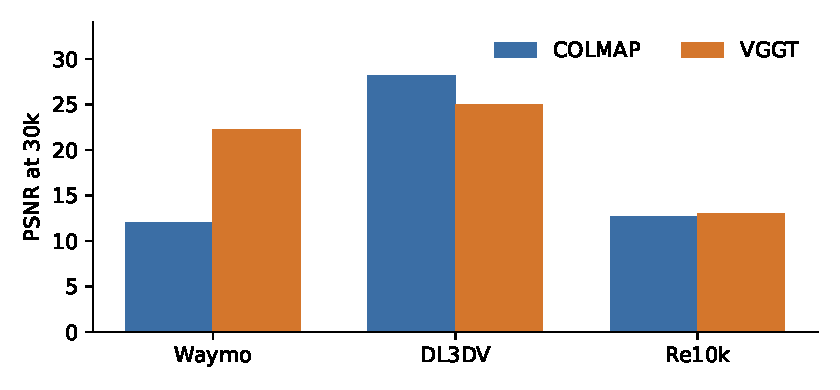
\includegraphics[width=\linewidth]{figures/part1_psnr.pdf}
\caption{Test PSNR after 30{,}000 frozen-pose 3DGS iterations. VGGT leads on Waymo. COLMAP leads on DL3DV. The two initializers are close on Re10k, and both stay near 13\,dB.}
\label{fig:part1}
\end{figure}

\begin{figure*}[t]
\centering
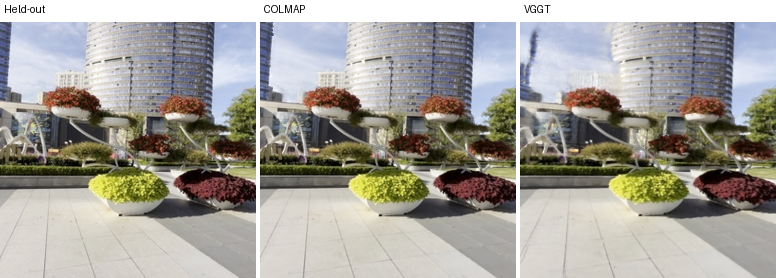
\includegraphics[width=\textwidth]{figures/part1_dl3dv.png}
\caption{DL3DV test frame 15 after the 500-step evaluation pose. Both initializers recover the plaza. COLMAP is the higher-scoring field (28.16\,dB against 25.03\,dB).}
\label{fig:dl3dv}
\end{figure*}

\begin{figure*}[t]
\centering
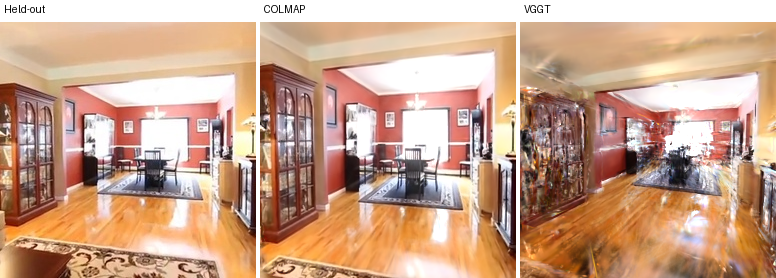
\includegraphics[width=\textwidth]{figures/part1_re10k.png}
\caption{Re10k test frame 15. COLMAP keeps the cabinet and the doorway. VGGT is within 0.4\,dB (13.02 vs.\ 12.69) and still warps the cabinet and the floor. PSNR does not show that failure.}
\label{fig:re10k}
\end{figure*}

On Waymo, VGGT is both faster to initialize and much more accurate.
COLMAP spends 10{,}450\,s, and its Sim(3) error is 4.02.
VGGT spends 237\,s and reaches pose error 1.12 and 22.25\,dB at 30k.
The COLMAP render is scored in the undistorted pinhole frame.
That removes the dataset distortion, but it does not repair a weak pose graph.
Extra 3DGS iterations do not help this COLMAP run: 30k is slightly below 7k.

On DL3DV the order reverses.
COLMAP initializes in 953\,s, pose error is 0.006, and 30k PSNR is 28.16\,dB with LPIPS 0.091.
VGGT's blocked forward takes 4712\,s, pose error rises to 0.035, and 30k PSNR is 25.03\,dB.
The first VGGT export of this scene kept zero points, because the default confidence threshold removed every depth sample.
3DGS then started from an empty cloud and aborted.
The reported VGGT row uses a second forward with threshold 0, which keeps 100{,}000 points, the same cap as the other scenes.
The camera estimate is still VGGT's.
Only the point filter changed.

On Re10k both initializers register every dense training view.
COLMAP is more accurate (ATE 0.011 vs.\ 0.066) and slightly better in LPIPS.
VGGT gains about 0.5\,dB from 7k to 30k and ends at 13.02\,dB, just above COLMAP's 12.69\,dB.
Figure~\ref{fig:re10k} shows why that ordering is not the whole result.
COLMAP renders the cabinet and the doorway.
VGGT bends the same cabinet and smears the floor.
The two errors have similar mean squared error and very different geometry.
Neither method moves far between 7k and 30k.
The indoor clip at $256\times256$ is a hard rendering target once the test frames are held out.
VGGT initialization is slow here, 4733\,s, because blocked global attention revisits keys for every query block.
That time is the price of fitting 270 frames on one 24\,GB GPU.
It is not comparable to Waymo's 237\,s joint forward.

\subsection{Part 2}
Table~\ref{tab:part2} scores the exported i3dgs models.
Figure~\ref{fig:part2} shows the same Re10k test frame from the sparse and dense exports.
The dense export is not a reconstruction of all 270 frames.
It is a field built from the six views i3dgs registered.

Dense training does not mean a dense pose graph.
On DL3DV, 271 of the dense views are dropped and 19 remain.
On Re10k, 264 of 270 dense views are dropped and 6 remain.
On Waymo, 114 dense views are dropped.
The sparse splits drop fewer views: 3 on Waymo, 0 on DL3DV, and 5 on Re10k.
Pose error on the views that remain can look small while the dropped count says the registration failed.
That is why the count is reported beside the error.

\begin{table}[t]
\centering
\small
\setlength{\tabcolsep}{3pt}
\begin{tabular}{llrrrrr}
\toprule
Scene & Split & PSNR & SSIM & LPIPS & ATE & Drop \\
\midrule
Waymo & sparse & 16.92 & 0.623 & 0.547 & 0.739 & 3 \\
Waymo & dense & 16.25 & 0.598 & 0.578 & 1.306 & 114 \\
DL3DV & sparse & 11.02 & 0.326 & 0.696 & 0.024 & 0 \\
DL3DV & dense & 10.81 & 0.371 & 0.572 & 0.010 & 271 \\
Re10k & sparse & 14.53 & 0.540 & 0.463 & 0.003 & 5 \\
Re10k & dense & 16.68 & 0.651 & 0.400 & 0.006 & 264 \\
\bottomrule
\end{tabular}
\caption{Part~2 i3dgs on the exported Gaussians. Joint time is 87\,s and 359\,s on Waymo sparse and dense, 57\,s and 108\,s on DL3DV, and 39\,s and 40\,s on Re10k. Registered counts are 17/20 and 65/179 on Waymo, 10/10 and 19/290 on DL3DV, and 5/10 and 6/270 on Re10k.}
\label{tab:part2}
\end{table}

\begin{figure*}[t]
\centering
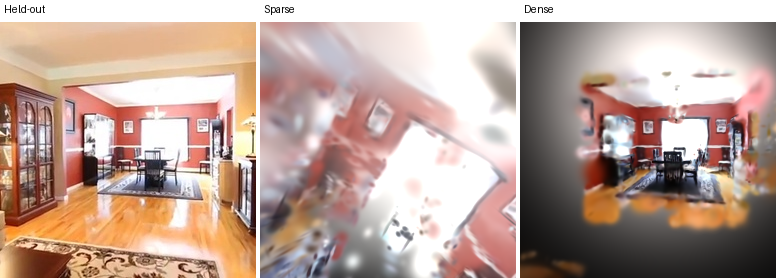
\includegraphics[width=\textwidth]{figures/part2_re10k.png}
\caption{Re10k test frame 15 from i3dgs after the same 500-step pose fit. Sparse keeps 5 of 10 views and does not land on this camera. Dense keeps 6 of 270, is recognizable, and does not fill the frame. Its higher score (16.68 vs.\ 14.53\,dB) is not evidence that the dropped frames were used.}
\label{fig:part2}
\end{figure*}

Sparse Waymo renders better than dense Waymo (16.92 vs.\ 16.25\,dB) and has a lower pose error.
Dense Re10k renders better than sparse Re10k (16.68 vs.\ 14.53\,dB) even though almost all dense frames are dropped.
The retained keyframes are enough for a coarse indoor field, and the extra images that never register do not enter the loss.
DL3DV stays near 11\,dB in both splits.
The sparse split registers every sparse training view.
The dense split's low pose error is computed on 19 cameras only.

These exports are not the Part~1 models.
Outlier Gaussians were removed so the rasterizer could run, and the scene was normalized.
The photometric numbers are therefore scores of the trainable i3dgs field, after that filter.

\subsection{Part 3}
Table~\ref{tab:part3} compares the sparse-only control with the closed loop.
All three scenes have both generation rounds.

\begin{table*}[t]
\centering
\small
\setlength{\tabcolsep}{3.2pt}
\begin{tabular}{llrrrrrr}
\toprule
Scene & Run & 1.5k & 3k & 4.5k & 7k & 30k & Recon.~s \\
\midrule
Waymo & control & 19.18 & 8.41 & 19.28 & 19.40 & 19.28 & 2685 \\
Waymo & loop & 19.14 & 8.46 & 15.25 & 15.18 & 14.96 & 1709 \\
DL3DV & control & 16.74 & 5.78 & 16.12 & 16.01 & 16.08 & 525 \\
DL3DV & loop & 16.60 & 5.86 & 9.18 & 10.61 & 12.60 & 514 \\
Re10k & control & 18.06 & 5.05 & 18.06 & 18.54 & 17.91 & 267 \\
Re10k & loop & 17.95 & 4.78 & 11.01 & 12.44 & 12.86 & 513 \\
\bottomrule
\end{tabular}
\caption{Part~3 test PSNR. Generation time is 150.6\,s on Waymo, 22.9\,s on DL3DV, and 24.3\,s on Re10k, and is not inside Recon. The 3k column is the opacity reset.}
\label{tab:part3}
\end{table*}

\begin{table}[t]
\centering
\small
\setlength{\tabcolsep}{4pt}
\begin{tabular}{llrrrr}
\toprule
Scene & Run & SSIM$_{7}$ & LPIPS$_{7}$ & SSIM$_{30}$ & LPIPS$_{30}$ \\
\midrule
Waymo & control & 0.679 & 0.471 & 0.641 & 0.470 \\
Waymo & loop & 0.648 & 0.587 & 0.586 & 0.600 \\
DL3DV & control & 0.485 & 0.417 & 0.476 & 0.427 \\
DL3DV & loop & 0.271 & 0.658 & 0.287 & 0.559 \\
Re10k & control & 0.690 & 0.233 & 0.662 & 0.260 \\
Re10k & loop & 0.397 & 0.498 & 0.396 & 0.469 \\
\bottomrule
\end{tabular}
\caption{Part~3 SSIM and LPIPS beside Table~\ref{tab:part3}. The loop remains worse on both metrics after 30k, not only on PSNR.}
\label{tab:part3b}
\end{table}

\begin{figure*}[t]
\centering
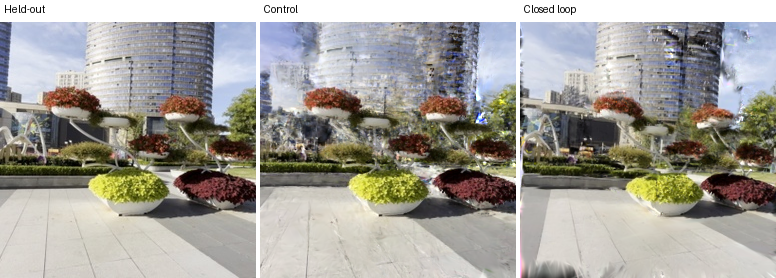
\includegraphics[width=\textwidth]{figures/part3_dl3dv.png}
\caption{DL3DV test frame 15 at 30k. The control still ghosts the tower and scores 16.08\,dB. The closed loop smears the tower and the lower edge and scores 12.60\,dB. Both are far below the dense COLMAP field in Figure~\ref{fig:dl3dv}.}
\label{fig:part3}
\end{figure*}

Every finished run drops at iteration 3000 and then recovers.
That iteration is the opacity reset in the 3DGS schedule, not a scoring bug.
The same dip appears on Waymo, DL3DV, and Re10k, and it appears in both the control and the loop.
Judging the generative method at 3000 would only measure the reset.

Figure~\ref{fig:part3} is the same DL3DV test frame from the control and from the loop at 30k.
The control keeps the planters and the tower.
The loop is blurrier and lower contrast, which is the same gap as the table: 16.08\,dB against 12.60\,dB.

On DL3DV the loop matches the control at 1500 (16.60 vs.\ 16.74\,dB) and then falls behind.
At 4500, after both generated rounds have been inserted, the loop is 9.18\,dB and the control is 16.12\,dB.
By 30k the loop has climbed to 12.60\,dB and the control is still 16.08\,dB.
Two rounds of GeoQuery, with equal photometric weight and no confidence mask, did not improve this sparse outdoor scene.
The generated views add observations that the frozen, interpolated poses do not explain well enough to help the test images.
The control never sees those observations and keeps the sparse field intact.
Dropped views for this sparse split are zero, so the gap is not an i3dgs registration failure.

Waymo's control ends at 19.28\,dB after 2685\,s, with three dropped sparse views and pose error 0.74.
Its loop matches that control at 1500 (19.14 vs.\ 19.18\,dB) and then falls behind: 15.25\,dB at 4500 and 14.96\,dB at 30k, against 19.28\,dB for the control.
Generation is 150.6\,s because the driving views are wide, and reconstruction is 1709\,s.
Re10k's control ends at 17.91\,dB after 267\,s, with five dropped views and pose error 0.0025.
The Re10k loop matches that control at 1500 (17.95 vs.\ 18.06\,dB), before the generated views are in the optimizer, and then falls behind.
At 4500 the loop is 11.01\,dB and the control is 18.06\,dB.
At 30k the loop is 12.86\,dB and the control is 17.91\,dB.
SSIM and LPIPS move the same way: the loop at 30k is 0.396 / 0.469 against the control's 0.662 / 0.260.
Generation for this loop is 24.3\,s and reconstruction is 513\,s.
The indoor scene repeats the DL3DV result.
Equal-weight GeoQuery views, on frozen interpolated poses, lower the test score.

\subsection{What the clocks say}
COLMAP is cheap on DL3DV and expensive on Waymo.
VGGT is cheap on Waymo, where 179 frames fit in one joint forward, and expensive on the longer scenes, where blocked attention is exact but quadratic in the number of blocks.
Reconstruction time tracks resolution and Gaussian count more than it tracks the initializer.
Waymo 3DGS takes about half an hour.
The $256\times256$ scenes finish the 30k loop in roughly seven to thirteen minutes.
i3dgs joint time stays under a minute on the sparse splits and on both Re10k splits, because most dense frames are dropped before they become keyframes.
Generation is 151\,s on Waymo and about 23\,s on the two $256\times256$ loops.
It is reported separately from the 3DGS time.

\subsection{Limits of the comparison}
VGGT-$\Omega$ is the missing third initializer.
The public file \texttt{vggt\_omega\_1b\_512.pt} is gated.
An unauthenticated download returns HTTP 401, and no poses were invented in its place.
A later run with access would use the same frozen-pose 3DGS budget, so the table can grow a row without changing the protocol.

The DL3DV VGGT cloud is also not the default export.
Confidence 5.0 left zero points, and 3DGS cannot start from an empty cloud.
The reported row keeps 100{,}000 points at confidence 0.
That choice can only help the point cloud.
It does not change the camera head.
The remaining gap to COLMAP is therefore not an empty-cloud failure.

Waymo generation does not run the UNet at 1600 pixels.
The first attempt allocated 3.25\,GiB with 0.6\,GiB free and stopped before any generated view was written.
The rerun restores at long side 512 and resamples to the camera size.
DL3DV and Re10k never hit that cap.
Their comparison with Waymo is still the same schedule, the same two rounds, and the same equal-weight loss, at different diffusion resolutions.

i3dgs dense runs should not be read as ``more views are worse.''
On DL3DV and Re10k almost every extra frame is dropped, so the dense and sparse fields are both sparse.
The useful comparison is the dropped-view count next to the pose error.
A Sim(3) error of 0.010 on 19 cameras is a different claim from the same error on 290 cameras.

The frames in Figures~\ref{fig:dl3dv}--\ref{fig:part3} use that same 500-step pose.
On Re10k the fit does not undo the VGGT warp, and it does not place the sparse i3dgs camera on the held-out frame.
The Adam step is $10^{-2}$ and the numeric difference is $10^{-3}$.
Those are the values behind every test number in the tables.
A longer fit could move the camera.
It would not fill the black border in the dense i3dgs render, because that border is missing scene content, not a one-pixel pose error.

The 3000-iteration column is reported because the schedule asks for it.
It is the opacity reset.
Every finished control and the DL3DV loop fall to about 5--8\,dB there and recover by 4500 when no new views have been added.
After the second generated round, the DL3DV loop does not recover to the control.
That later gap is the result of the generative views.

Initialization time and reconstruction time are stored as separate clocks and are never added.
On Waymo, COLMAP spends 10{,}450\,s before 3DGS starts, while VGGT spends 237\,s.
On DL3DV and Re10k the blocked VGGT forward is the slow clock, 4712\,s and 4733\,s, and the later 3DGS loop is a few hundred seconds.
Generation is 150.6\,s on Waymo, 22.9\,s on DL3DV, and 24.3\,s on Re10k.
Joint i3dgs time stays under a minute except for dense Waymo (359\,s), because frames that never become keyframes do not enter the Gaussian optimization.
A single ``runtime'' number would hide which stage actually cost the time.

\section{Conclusion}
Feed-forward initialization is not uniformly better than COLMAP.
On the outdoor driving scene, VGGT produces a usable pose graph in a few minutes and COLMAP does not.
On DL3DV, COLMAP remains the better initializer by several decibels.
On the small indoor scene the two are close, and both leave a large perceptual error.
VGGT-$\Omega$ was not compared.
The gated checkpoint is a missing experiment, not a negative result.

i3dgs should be read together with the dropped-view count.
A low pose error on a handful of registered frames does not mean the dense video was reconstructed.
Sparse inputs are the setting in which registration succeeds.

The closed loop does not beat a sparse-only control that uses the same Gaussians and the same frozen poses, on any of the three scenes.
The 3000-iteration opacity reset creates a temporary collapse that should not be interpreted as a property of GeoQuery.
The later gap, from 4500 through 30k, is the informative one, and it favors the control.

VGGT-$\Omega$ remains ungated access away from a third initializer row.
Optional datasets were not run.
The mandatory scenes already show that the ranking of initializers depends on the scene, and that unfiltered generated views can hurt a sparse Gaussian field.

{\small
\bibliographystyle{ieeenat_fullname}
\bibliography{refs}
}

\end{document}
